
\documentclass[a4paper, 12pt]{report}

\usepackage[T1]{fontenc}
\usepackage[dvips]{epsfig}

\usepackage[latin1]{inputenc}

\usepackage[english]{babel}
\usepackage{times}
\usepackage[dvips]{graphics}

\usepackage[]{vmargin}
\usepackage{url}
\usepackage[]{longtable}

\usepackage{natbib}
\bibpunct{(}{)}{;}{a}{,}{,}

\newcommand{\jel}{Jeliot 3}
\newcommand{\djava}{DynamicJava}
\newcommand{\mcode}{MCode}
\newcommand{\andres}{Andr\'{e}s}
%--\def\@minstr#1{\begin{tabular}[t]{@{}l@{\extracolsep{\fill}}}#1\end{tabular}} 
\newcommand{\minstr}[1]{
 \begin{tabular}{|p{30em}|}
 \hline
 \p{#1}\\ 
 \hline
	\end{tabular}\par
}
%  Alternative minstr
%\newcommand{\minstr}[1]{
%	\framebox[32em]{\parbox[t]{31em}{\p{#1}}}
%}
%\framebox[\textwidth][c]
%\newenvironment{minstr}%
%    {\nopagebreak\par\small\addvspace{3.2ex plus 0.8ex minus 0.2ex}%
%     \vskip -\parskip
%     \noindent%
%     \begin{tabular}{|l|}\hline\rule{0pt}{1em}\ignorespaces}%
%    {\\\hline\end{tabular}\par\nopagebreak\addvspace{3.2ex plus 0.8ex
%        minus 0.2ex}%
%     \vskip -\parskip}
\newcommand{\p}[1]{\texttt{#1}}
\newcommand{\bu}[1]{\textsf{#1}}
\newcommand{\f}[1]{\textsf{#1}}


\setlength{\parindent}{0pt} \setlength{\parskip}{2ex}
\linespread{1.0}
%\sloppy
%\fussy

\setpapersize{A4}
\setmarginsrb{35mm}{30mm}{30mm}{20mm}{0pt}{0mm}{12pt}{13mm}


\title{\jel{} Intermediate Code Specifications\\\mcode{}}
\author{Niko Myller and \andres{} Moreno Garc\'{\i}a}
%\date{}

\begin{document}
% ----------------- Coverpage -------------------------------

\maketitle
\thispagestyle{empty}

\newpage

\thispagestyle{empty} % no page numbering
\vfil
Copyright 2003 by Niko Myller and Andr\'{e}s Moreno Garc\'{\i}a.
\bigskip

This document is to be considered as part of the program
\emph{\jel} and can be used under the same terms.
\bigskip

{\small
This program is free software; you can redistribute it and/or
modify it under the terms of the GNU General Public License
as published by the Free Software Foundation; either version 2
of the License, or (at your option) any later version.
This program is distributed in the hope that it will be useful
but WITHOUT ANY WARRANTY; without even the implied warranty of
MERCHANTABILITY or FITNESS FOR A PARTICULAR PURPOSE.
See the GNU General Public License for more details.
You should have received a copy of the GNU General Public License
along with this program; if not, write to the Free Software
Foundation, Inc., 59 Temple Place - Suite 330, Boston, MA
02111-1307, USA.
}

\vfil
\newpage

% ----------------- Generation of Table of Contents -------------

\thispagestyle{empty} % no page numbering

\setlength{\parskip}{0ex}

\tableofcontents
\newpage

\setlength{\parskip}{2ex}

% ----------------- Document begins ------------------------

\setcounter{page}{1}

\pagenumbering{arabic} % page numbering with arabic numbers

%Introduction
\section{Introduction}
\label{sec:Introduction}

\jel{} is a program animation system intended for teaching introductory
programming. Programs are animated fully or semi-automatically, requiring
no modifications or annotations on the part of the instructor or student.
While this limits the flexibility of the animation, \jel{} is extremely
simple to use so that it is easily accepted by true novices, as well as
by their teachers who do not have to invest in learning how to prepare
animations.

\jel{} is written in Java for portability and animates program that are
written in Java. \jel{} uses a modified version of \djava{} \citep{DJava}
(section~\ref{sec:DynamicJava}) as a front-end and
modified version of \jel{}~2000's animation engine
(section~\ref{sec:Visualization_Engine}) as its back-end. The user interface
was also adopted from \jel{}~2000 (sections~\ref{sec:Jeliot_Class} and
\ref{sec:User_Interface}).

\djava{} is a Java source code interpreter written in Java. This
application is open source and can be freely obtained from
\url{http://www.koala.ilog.fr/djava/}. At the moment, DynamicJava is
almost fully compliant with Java language specifications and supports
multi-threading.

To make these two separate systems communicate
(section~\ref{sec:Communications_Model}) with each other a new
intermediate code (section~\ref{sec:Intermediate_Code} and
Intermediate Language Specification) and intermediate code
interpreter (section~\ref{sec:Intermediate_Code_Interpreter}) were
designed. In this way the system should be more flexible for
modifications and new extensions
(sections~\ref{sec:Managing_Jeliot_3_System} and
\ref{sec:Extending_Jeliot_System}).

\subsection{History}

The first member of the \jel{} family of program animation systems was
called Eliot; it was developed by Erkki Sutinen and Jorma Tarhio and
their students at the University of Helsinki. Eliot was written in C
and used the Polka animation library. Later a version was written in
Java and the name was changed to \jel{}. (This version is now called
\jel{}~I to distinguish it from later versions.)

\jel{}~I was a flexible system: the user could choose the variables to
be animated, the graphical form of the animated elements and multiple
views of the same program. It proved too difficult for teaching novices,
so a new version called \jel{}~2000 was developed at the Weizmann Institute
of Science by Pekka Uronen under the supervision of Moti Ben-Ari.
A pedagogical experiment carried out by Ronit Ben-Bassat Levy proved
the effectiveness of \jel{} in teaching introductory programming.

\jel{}~2000 only implemented a very small subset of the Java language.
The current version \jel{}~3 is a re-implementation designed to
significantly extend the range of Java features that are animated,
in particular, to cover object-oriented programming. The design and
implementation was carried out at the University of Joensuu by
Niko Myller and Andr{\'{e}} Moreno-Garc{\'{\i}}a, under the supervision
of Moti Ben-Ari and Erkki Sutinen. For an extensive discussion of the
history of \jel{}, see \citep{Benari2002a}.

\subsection{Release Notes}
\label{sec:Release_Notes}

\paragraph{version 3.2} contains documentation and supports
inheritance, supports: inheritance of classes and \p{super()}
method calls at the beginning of a constructor.

\paragraph{version 3.1} supports objects creation and object method
calls. Line numbering was added for source code editor and viewer.
Supports:
\begin{itemize} \item User made classes, however,
inheritance is not yet supported. \item Constructor calls. \item
Object method calls. \item Object field access.
\end{itemize}


\paragraph{Version 3.01} is a maintenance release. Bugs of the initial
release were fixed. Support for \p{switch} statement was added.

\paragraph{Version 3.0} is the initial public release. Supports:
\begin{itemize}
\item Values of type \p{String}, all primitive types. \item
One-dimensional arrays with primitive types or strings as its
component type. \item Expressions including all unary and binary
operations except \p{instanceof}. \item All the control statements
(\p{if}, \p{while}, etc.) except \p{switch} statement and
conditional expression (\p{exp?exp1:exp2}). \item Method
invocation, including recursive invocation.
\end{itemize}

\paragraph{Not implemented:}
\begin{itemize}
\item Static variables. \item Calls to \p{super()} with
parameters. \item Super field accesses. \item Arrays with
components of reference type (except \p{String}). \item
Conditional expressions (\p{exp?exp1:exp2}). \item Array
initializers. \item Java 2 SDK API classes' methods cannot return
object or array types.
\end{itemize}

\newpage

\chapter{Overall Description}
\label{ch:overall}

\section{\jel{} System Structure}
\label{sec:structure}
\includegraphics[height=10cm]{communicationmodel.eps}
\section{\mcode{} functions}
\label{sec:functions}
\mcode{} is the intermediate language used to communicate the visualization engine and the Java interpreter (\djava{}). It mainly flows from \djava{}to the Director.  The information that carries along within is not only the information about modified variables and modified method stacks, but also the operations that produce such changes. and the results of those operations. This is the biggest difference from normal compiler intermediate codes; they only indicate what operations to perform to the assembler. In our case all operations are performed and the every result is sent to the Director.

\section{User Characteristics}
\label{sec:users}

This document is addressed to the following people:

\begin{description}
	\item[Developer of Visualization Systems] This document may provide ideas and solutions to developers of new visualization systems, as well as provides of an existing solution that can be merged into their ongoing projects.
	
	\item[Maintainer of \jel{}] Future developers and maintainers of \jel{} should refer to this document when modifying its source code, specially those files referring to \djava{} and \jel{}'s interpreter. They should incorporate here all changes done to \mcode{} to provide a state of the art document as well. 
	
\end{description}

\section{Features and Constraints}
\label{sec:features}

While trying to produce the more generic intermediate code some features and constraints where placed due to several reasons. The most important ones are the following ones:

\begin{description}
	\item[Java] Being Java the language of choice, \mcode{} supports most of its characteristics and abilities. It is object oriented, so things as method calls, objects and, to some extend, inheritance are supported.
	
	\item[\djava{}]Because of using \djava{} as an interpreter from which to extract the execution information, some of the specified ordered sequences of instructions may be too constrained to the particularity of \djava{}. However that is not the case for the most of instructions explained here.
	
	\item[Targeted audience] \mcode{} was designed to support the development of \mcode{}, thus it was important to address their specific problems: \mcode{} has a great detail in the evaluation of expressions and the normal flow of program, so novices will grasp the programming fundamental issues. Meanwhile, more advanced features are not within the scope of the \mcode{} and have not been implemented. Those features include threads, reflection utilities and exception handling. 
	
\end{description}

\section{Dependencies}
\label{sec:dependencies}

Right now \mcode{} is only produced through the modified version of \djava{} included in the distribution of \jel{}. However it is up to anyone to create a new high\-{}level interpreter to produce its own \mcode{} to be run by \jel{}'s \mcode{} interpreter or by one they develop. 
There is also the possibility to store the \mcode{} a single text file and be retrieved later by a \mcode{} interpreter to produce visualization orders. However, this configuration would not allow INPUT/OUTPUT operations as they provide information to the evaluation needed to carry on with following instructions. 
\newpage


\chapter{MCode Language}
\label{ch:MCode}

\section{Introduction}
\label{sec:Introduction}

\mcode{} is defined to be an interpreted line by line and each line can be divided in the smaller pieces or tokens. Here we define all the commands that are part of \mcode{}.
First of all, we will introduce the notation used in this specification. as it is not standard. In our notation each token is now separated by single '\p{�}' character, this token will not be shown here instead a blank space will be used to help readability. Each token is first introduced as an English name. Later a sample instruction is given, consisting of the different tokens that build that particular instruction. If the token is in big letters it is a preserved word. If it is in small letters it will be replaced by variable value or integer.
Table~\ref{tab:token_abbreviations} shows the abbreviations used in the specification to refer to some common tokens:

\begin{table}[htbp] 
\begin{tabular}{|p{11.5em}|p{3em}|p{16.5em}|}
\hline
 Name                       & Ab\-bre\-vi\-a\-tion & Meaning \\\hline 
 Instruction Reference      & \p{ir}       & Used to keep track of instructions used in the past.\\\hline 
 Left Instruction Reference  & \p{lir}      & A reference to a previous instruction used as the left operand.\\\hline 
 Right Instruction Reference & \p{rir}      & A reference to a previous instruction used as the right operand. \\\hline 
 Instruction Counter         & \p{ic}       & Counter of expressions, making instructions unique and easily referenciable \\\hline 
 Type of instruction         & \p{ti}       & Refer to some m-code instruction (e.g. \p{ADD})\\\hline 
 Location                    & \p{lo}       & Variable that holds the location of the expression in the source code, defined by ``beginning of line'', ``beginning of column'', ``end of line'', ``end of column''.\\\hline 
\end{tabular}
\caption{Token Abbreviations.} 
\label{tab:token_abbreviations} 
\end{table}

The usual \mcode{} sentence will consist of:

\begin{description}

	\item{\p{Expression/Statement code}} A shortcut for every Java statement or expression is used: e.g. AE stands for Add Expression. The chosen names are heavily related to the ones used in \djava{}.
	
	\item{\p{Reference}} Every Expression/Statement sentence is identified by a number. This way nested statements and expressions can be formed up from previous m-code sentences.
	
	\item{\p{Related References}} Most of the m-code sentences refer to previous m-code sentences. One Add Expression will refer to the references of both sides of expression. Flow-control statements will refer to a condition expression, and so on.
	
	\item{\p{Value}} Most sentences will return the value resulting from the executing of an expression. If it is a flow control statement it will return a Boolean value indicating the result of the condition.
	
	\item{\p{Type}} Every expression that has a result must specify its type.
	
	\item{\p{Location}} This contains the location of the expression in the original source code file.
	
\end{description}

\section{Grammar}

The following grammar expresses the syntactic properties of the \mcode{}. It describes how to get a sintactically correct \mcode{} program, that can be parsed by the interpreter provided \jel{} to produce the right visualizations. This grammar has been obtained by modifying the Java BNF sintactic grammar.

Tokens within "<" and ">" are Non-Terminal symbols, capitalized words are Terminal symbols, basically \mcode{} commands; you will find a more detailed description of them in the follwing section."$?$" means that the preceeding symbol is optional, and "|" separates the different possibilities.

<program> ::= <classes info> <static method call> \p{END}\footnote{The beginning Static Method Call it is supposed to call the Main method of the program}
\begin{tabbing}
<classes info> ::= \=<class info> \\
				\> | <classes info> <class info>
\end{tabbing}

<class info> ::= \p{CLASS METHOD CONSTRUCTOR FIELD}$?$  \p{END\_CLASS}
%<class info> ::= \p{CLASS} \p{METHOD} \p{CONSTRUCTOR} \p{FIELD}? \p{END_CLASS}


<static method call> ::= \p{SMC} <method call info> <method body> \p{SMCC}

<object method call> ::= \p{OMC} <method call info> <method body> \p{OMCC}

<method call info> ::= \p{PARAMETER} \p{MD} <parameters info>?
\begin{tabbing}
<parameters info> ::= \=<parameter info> \\
					  \> | <parameters info> <parameter info>
\end{tabbing}
<parameter info> ::= \p{BEGIN} <expression> \p{P}

<method body> ::= <block statements>
\begin{tabbing}
<block statements> ::= \= <block statement> \\
					   \>| <block statements> <block statement>
\end{tabbing}
\begin{tabbing}					   
<block statement> ::= \= <variable declaration> \\
                      \> | <statement>
\end{tabbing}
<scoped block> ::= \p{SCOPE 1} <block statements> \p{SCOPE 0}

\begin{tabbing}
<statement> ::= \= <simple statement> \\
				\> | <if statement> \\
				\> | <for statement> \\
				\> | <while statement> 
\end{tabbing}
\begin{tabbing}				
<simple statement> ::= \= <scoped block> \\
					\> | <statement expression> \\
					\> | <switch statement> \\
					\> | <do statement> \\
					\> | <continue statement> \\
					\> | <break statement> \\
					\> | <return statement>
\end{tabbing}
\begin{tabbing}					
<statement expression> ::= \= <assignment> \\
						   \> | <pre expression> \\
						   \> | <post expression> \\
						   \> | <method call> \\
						   \> | <class allocation>
\end{tabbing}
\begin{tabbing}
<if statement> ::= \= <expression> \p{IFT} <statement>? \\
				   \> | <expression> \p{IFTE} <statement>? 
\end{tabbing}				  
<while statement> ::= <expression> \p{WHI} <statement>?

<switch statement> ::= \p{SWITCHB} <expression> \p{SWITCHBF} <block>? \p{SWITCH}

<for statement> ::= \p{SCOPE 1} <variable declarations> <expression> \p{FOR} <statement>? \p{SCOPE 0} 

<do statement> ::= <block> <expression> \p{DO}

<break statement> ::= \p{BREAK}

<break statement> ::= \p{CONTINUE}

<return statement> ::= <expression>? \p{RETURN}

\begin{tabbing}
<expression> ::= \= <assignment> \\
				 \> | <binary expression> \\
				 \> | <unary expression> \\
				 \> | <primary>
\end{tabbing}
<assignment> ::=  \p{BEGIN} <expression> \p{TO} <left hand side>
\begin{tabbing}
<left hand side> ::= \= <identifier> \\
					 \> | <field access> \\
					 \> | <array access>
\end{tabbing}

<binary expression> ::= \p{BEGIN} \p{LEFT} <expression> \p{RIGHT} <expression> <binary operator>

<unary expression> ::= \p{BEGIN} <expression> <unary operator>
\begin{tabbing}
<primary> ::= \= <literal> \\
			  \> | <field access> \\
			  \> | <array access> \\
			  \> | <class allocation> \\
			  \> | <array allocation> \\
			  \>| <method call> 
\end{tabbing}
<literal> ::= \p{L}

<identifier> ::= \p{QN}

<variable declaration> ::= \p{VD}

<field access> ::= <primary> <identifier> OFA

<array access> ::= <identifier> <dim expressions> AAC
\begin{tabbing}
<dim expressions> ::= \= <expression> | \\
					  \> <dim expressions> <expression>
\end{tabbing}
\begin{tabbing}					  
<method call> ::= \= <static method call> \\
				  \> | <object method call>
\end{tabbing}
<array allocation> ::= <dims expressions> \p{AA}

<class allocation> ::= \p{SA} <method call info> <method body> \p{SAC}

\begin{tabbing}
<variable declarations> ::=\= <variable declaration> \\
						   \> | <variable declarations> <variable declaration>	   
						  						   
\end{tabbing}

<pre expression> ::= <identifier> \p{PRIE} | <identifier> \p{PRDE}

<post expression> ::= <identifer> \p{PIE} | <identifier> \p{PDE}

\begin{tabbing}
<unary operator> ::= \p{PLUS} | \p{MINUS} | \p{COMP} | \p{NO} 
\end{tabbing}
\begin{tabbing}
<binary operator> ::=\= \p{AE} | \p{SE} | \p{ME} | \p{DE} | \p{RE} \\
				     \> | \p{BITOR} | \p{BITXOR} | \p{BITAND} \\
				     \> | \p{LSHIFT}| \p{RSHIFT} | \p{URSHIFT} \\
				     \> | \p{XOR} | \p{AND} | \p{OR} | \p{EE} | \p{NE} \\
				     \> | \p{GT} | \p{LE} | \p{LQE} | \p{GQT} \\
\end{tabbing}
%\end{mcodegrammar}

\section{Constants}
\label{sec:constans}

Table~\ref{tab:constants} contains the constants used in the implementation of \mcode{} to support portability and maintainability.

\begin{table}[htbp] 
\begin{tabular}{|p{8em}|p{23em}|}
\hline
Constant          & Meaning \\\hline 
\p{DELIM}         & Used to separate tokens on a single instruction. They have to be explicitly added to the m-code instruction\\\hline 
\p{LOC\_DELIM}    & Used to separate the different coordinates that locate some source code.\\\hline 
\p{UNKNOWN}       & When some variable value cannot be accessed it is given an \p{UNKNOWN} value.\\\hline 
\p{NO\_REFERENCE} & ?? \\\hline 
\p{REFERENCE}     & ?? \\\hline 
\p{NOT\_FINAL}    & ?? \\\hline 
\p{FINAL}         & ?? \\\hline 
\p{TRUE}          & String that represent the \p{TRUE} Boolean value in the working environment.\\\hline 
\p{FALSE}         & String that represent the \p{FALSE} Boolean value in the working environment.\\\hline 
\end{tabular}
\caption{Constants.} 
\label{tab:constants} 
\end{table}

\section{Auxiliary Instructions}
\label{sec:auxiliary}

Some auxiliary instructions are defined in order to ease the interpretation of the m-code. These instructions are not related to any particular Java construct and are used by those that need them.

\subsection{BEGIN}

\minstr{BEGIN ti ir loc}

Instruction used to mark the beginning of those instructions that admit instructions to be encapsulated within them. Those instructions are Assignment, Return, Parameter, Array Access and all unary and binary operations; and they are referred through it. The referred instructions get they \p{ir} assigned in the \p{BEGIN} instruction.

\subsection {LEFT and RIGHT}

\minstr{LEFT/RIGHT ir}

These instructions are similar to \p{BEGIN}. Both of them are used to mark the beginning of the \p{left}/\p{right} side of a binary operation. The \p{ir} obeys the same reason than in \p{BEGIN}, ``reserves'' the reference number for the following instruction.

\subsection {TO}

\minstr{TO ir}

This instruction is used in assignments and reflects the movement of the value to the left hand side of the assignment. The \p{ir} points to the qualified name that will hold the value. As said before, this instruction is used in assignment and more concretely in Assignment, Variable Declaration (those with initializer) and Compound Assignment.

\subsection {ERROR}

\minstr{ERROR errorMessage loc}

Parser and execution errors are reported to the visualization engine with the \p{ERROR} instruction. The \p{errorMessage} is a string that can contain \p{HTML} and it is what will be visualized.

\subsection {END}

\minstr{END}

END is produced at the end of the \mcode{} program and indicates the visualization to terminate. 

\subsection {SCOPE}

\minstr{SCOPE 1/0}

New blocks of Java code are delimited in \mcode{} through \p{SCOPE}. This instruction second token indicates whether it is opening a new one (\p{1}) or closing one (\p{0}).

\subsection {CONSCN (Constructor Call Number)}

\minstr{CONSCN ir}

CAUTION! This instruction is implementation specific and the need for the usage of this instruction depends on the implementation of the interpreter. If your interpreter traverses the tree in the right order there is no need to use the \p{CONSCN}. The usage of the instruction is next described in \djava{}.

This instruction is created because in \djava{} the super method calls in the beginning of the constructor
are handled before the actual constructor invocation and thus the information is not extracted in the correct order. The constructor call number is used to correct the order so that during the simple allocation visit in EvaluationVisitor the constructor call number is send for the first time. When all the super method calls are finished and the constructor is really invoked the constructor call number is printed out again. The \mcode{} interpreter collects all the commands between the corresponding constructor call numbers and executes them after the constructor is really invoked that is two lines after the second constructor call number is read.
However this instruction is due to \djava{} drawbacks. If your interpreter traverses the tree in a meaningful way, you should not use the CONSCN instruction.

\section{Statements}

\subsection{A (Assignment)}

\minstr{A ir rir lir value type loc}

The assignment instruction is composed by its own reference (\p{ir}) and the references to the left and right hand sides (\p{lir}, \p{rir}). Furthermore it contains the assigned value and its type.

It is worth to mention that compound assignments are decomposed into the operation and a simple assignment.

\subsection{VD (Variable Declaration)}

\minstr{VD name NO\_REFERENCE/ir value type FINAL/NOT\_FINAL loc}

When declaring a variable the corresponding the \mcode{} instruction needs to be complemented with its name, value, type and the modifier (\p{FINAL} or \p{NOT\_FINAL}). Instruction reference (\p{ir}) is given if the variable has an initializer otherwise a \p{NO\_REFERENCE} value is written. 

\section{Binary Operations}

\minstr{binaryCode ir rir lir value type loc}

Binary instructions are composed by its \p{binaryCode}, its own reference (\p{ir}) and the references to the left and right sides of the expression (\p{lir}, \p{rir}). Furthermore, it contains the assigned \p{value} and its \p{type}. The \p{binaryCode} can take any of the values shown in Table~\ref{tab:BinaryOperators}

\begin{table}[htbp]
	\centering
	\caption{Binary Operators that can be assigned to the \p{binaryCode}.}
	\label{tab:BinaryOperators}
		\begin{tabular}{|p{6em}|p{3em}||p{6em}|p{3em}||p{5.5em}|p{4em}|}
		\hline
		Boolean operators  & \mcode{}     & Arithmetic operators & \mcode{}    & Bitwise operators & \mcode{}\\\hline\hline
		AND \verb|&&|   & \p{AND}     & ADD +              & \p{AE} & AND \verb|&|              & \p{BITAND}\\\hline
		OR \verb$|$     & \p{OR}      & SUBTRACT \verb|-|  & \p{SE} & OR \verb$|$               & \p{BITOR}\\\hline
		XOR \verb|^|    & \p{XOR}     & MULTIPLY *         & \p{ME} & XOR \verb|^|              & \p{BITXOR}\\\hline
		LESSER THAN <   & \p{LE}      & DIVIDE  /          & \p{DE} & LEFT SHIFT \verb|<<|      & \p{LSHIFT}\\\hline
		GREATER THAN >  & \p{GT}      & REMAINDER \verb|%| & \p{RE} & RIGHT SHIFT \verb|>>|     & \p{RSHIFT}\\\hline
		EQUAL ==        & \p{EE}      &                    &        & UNSIGNED SHIFT \verb|>>>| & \p{USHIFT}\\\hline
		NOT EQUAL !=    & \p{NE}              & & & & \\\hline
		LESSER THAN OR EQUAL TO >=  & \p{LQE} & & & & \\\hline
		GREATER THAN OR EQUAL TO =< & \p{GQT} & & & & \\\hline
		\end{tabular}
\end{table}

\section{Unary Operations}

\minstr{unaryCode ir reference value type loc}

As with binary operations the unary instructions (\p{unaryCode}) take the similar tokens. The only difference is that there is only one \p{reference} to another instruction. The \p{value}, \p{type} and \p{loc} maintain the same meaning. As before there are several Java unary operators that can be assigned to the \p{unaryCode}, all of them are listed in Table~\ref{tab:UnaryOperators}.

\begin{table}[htbp]
	\centering
	\caption{Unary Operators that can be assigned to the \p{unaryCode}.}
	\label{tab:UnaryOperators}
	\begin{tabular}{|p{6em}|p{3em}||p{6em}|p{3em}||p{6em}|p{3em}|}
		\hline
		Boolean Operators & \mcode{} & Arithmetic operators & \mcode{} & Bitwise operators & \mcode{} \\\hline\hline
		NOT ! & NO & POST\-IN\-CRE\-MENT ++        & PIE   & COM\-PLE\-MENT \verb|~| &  COMP \\\hline
          &    & POST\-DE\-CRE\-MENT \verb|--| & PDE   &                         & \\\hline
          &    & PRE\-IN\-CRE\-MENT ++         & PRIE  &                         & \\\hline
          &    & PRE\-DE\-CRE\-MENT \verb|--|  & PRDE  &                         & \\\hline
          &    & PLUS +                        & PLUS  &                         & \\\hline
          &    & MINUS -                       & MINUS &                         & \\\hline
	\end{tabular}
\end{table}

\section{Literal constant and variable access}

\subsection{Qualified Name}

\minstr {QN ir name value type}

Qualified names are all the local variables. \mcode{} instruction contains the reference (\p{ir}) of the instruction and the name value and type of the qualified name. If the variable is not initialized value will be \p{UNKNOWN}.

\subsection{Literal}

\minstr{L ir value type loc}

Literals are the constants values in the source code (e.g. \p{3} is one integer literal and ``3'' is one string literal). The \mcode{} instruction contains all the information needed for the visualization as well as its reference (\p{ir}), \p{value}, \p{type} and \p{loc}. 

\section{Control Structures}

\subsection{If Statements}

\minstr{IFT/IFTE condition value loc}

There are two possible instructions for an ``If'' statement. \p{IFT} is printed if there is not an else statement or \p{IFTE} if there is an else statement. The composition, however, is similar. The \p{condition} is the reference to the instruction that evaluate the condition. The \p{value} holds the result of the evaluated condition and will tell which branch execution is following. The \p{loc} as usual contains the code location.

\subsection{While For and Do-While Statements}

\minstr{WHI/FOR/DO condition value round loc}

These statements produce a similar to the previous one. They only differ in the round token. This token holds the number of iterations the loop has made.

\subsection{Switch}

Three \mcode{} instructions are related to the switch statement.

\minstr{SWITCHB loc}

Switch statement interpretation begins with this instruction. The location of the whole switch block is given as the parameter.

\minstr{SWIBF selector ir loc}

The \p{SWIBF} instruction is written when one of the cases is selected as the matching case. The selector gives a reference to the selector expression. The instruction reference gives the reference for the case expression. If the default case is selected then the instruction reference is set to \p{-1}. The location explains the location of the found case block.

\minstr{SWITCH loc}

This statement is used when the switch statement is exited if the break instruction (\p{BR}) is not given. The parameter for \p{SWITCH} instruction is the location of the whole switch block.

\subsection{Break and Continue}

\minstr{BR/CONT statement loc}

Break and continue asserts instructions only specify which statement they are in. The allowed values for \p{statement} are \p{WHI}, \p{FOR}, \p{DO} or \p{SWITCH}.

\section{Input and Output}

\subsection{Input}

\minstr{INPUT ir type loc}

The \p{INPUT} instruction indicates the visualization engine to produce some data of the type specified and return it to Java interpreter. This data will be written in a dedicated pipe that connects both sides. The next instruction indicates the obtained value from the pipe.

\minstr{INPUTTED counter value type loc}

\subsection{Output}

\minstr{OUTPUT ir value type breakLine loc}

\p{OUTPUT} instruction is the resulting one of a call to any of the Output methods provided by \jel{} or System.out.print and System.out.println. They only accept one argument, and it is reflected in the instruction by its value and its type. A flag (\p{breakline} is added to indicate wheter to break the line (value \p{1}) or not (value \p{0}) in the output.

\section{Array Handling}

\subsection{Array Allocation}

\minstr{AA dimension dimensionsReferences dimensionsSizes loc}

Array allocation instruction is a complicated one, as it carries a lot of information about the array. As usual a \p{ir} is provided. Following the \p{arrayHashCode} of the object created to allocate it. It can be any other number that identify one-to-one the allocated object on the interpretation. The \p{type} contains the type of the array components. The \p{dimensionReferences} is a comma separated list with the references to the instructions that evaluated the sizes' expressions of the array. Finally, the \p{dimensionsSize} is another comma separated list where each element is the size of a dimension. An expression ``\p{new Integer[4][5]}'' will produce a following line of \mcode{} ``\p{AA ir 456744 Integer 2 ir1,ir2 4,5 loc}''. Where \p{ir1} and \p{ir2} must be references to the literal instructions of ``4'' and ``5'' respectively.

\subsection{Array Access}

\minstr{AAC ir arrayNameReference deep cellReferences cellNumbers value type loc}

Array accesses instructions consist on different tokens. The common ones (\p{ir}, \p{value}, \p{type} and \p{loc}) are also present. But we can find very specific ones.

The \p{arrayReference} points to the instruction produced when visiting an array name, normally a qualified name. deep refers to the level of deepness of the array access. This is useful for multidimensional arrays when they are not accessed till the last level, the one holding the data value. The \p{cellReferences} and the \p{cellNumber} meet the same purpose than \p{dimensionReferences} and \p{dimensionsSizes} in array allocation (\p{AA}) instruction. The \p{cellReferences} points to the instructions that evaluated the value of each cell pointer. The \p{cellNumbers} are the actual values of the cell access. Both of them are presented as a comma separated list. For example in ``\p{array[3][5]}'', \p{cellReferences} will point to the literal instruction of ``3'' and ``5'' and \p{cellNumbers} will contain ``3,5''.

\subsection{Array Length}

\minstr{AL objectCounter "length" value type loc}

\section{Object Oriented}

This section contains the instruction related to methods and object oriented programming. Here we will just summarize its properties and main arguments. However, following chapters will explain you how to glue the different instructions together to form meaningful \mcode{} programs.

\subsection{Parameters}

\minstr{PARAMETERS parameterArray}

The \p{PARAMETERS} instruction will provide the visualization engine a list of the types of the parameters used in the method declaration.

\minstr{P ir loc}

This instruction declares a new parameters in a method call.

\subsection{Method Declaration}

\minstr{MD ir loc}	

A method declaration instruction will indicate the location of the called method code and the beginning of its evaluation.

\subsection{Static Method Call}

\minstr{SMC name declaringClassName numArgs loc}

The \p{SMC} instruction consists of the actual name of the method, its declaring class name and the number of arguments this method call consists of.

\minstr{SMCC}

This instruction indicates the end of a call to a static method.

\subsection{Object Method Call}

\minstr{OMC name numArgs objectReference loc}

The \p{OMC} instruction is similar to the static method one. However it contains a reference to an object, this reference points to the instruction that holds the variable access to the object that is making the method call.

\minstr{OMCC}

As before it just closes the object method call.

\subsection{Class Allocation}

\minstr{SA ir declaringClass constructorName numArgs loc}

The class allocation instruction happens every time a \p{new} appears on the source code. It will provide the information needed for the constructor: declaring class, constructor name and the number of arguments it is being called with.

\minstr{SAC ir ObjectId loc}

\subsection{Object Field Access}

\minstr{OFA ir objectReference name value type loc}

This instruction accesses to the value of an object field, thus it references to the instruction that evaluate the object (objectReference) (normally a Qualified Name (\p{QN} one). It contains the name, the type and the value of the accessed field.

\subsection{Return}

\minstr{R callIr loc}

This first return instruction is just used for the "void" return, those that does not return anything. The \p{callIr} is the reference for the return value of the method and thus connect the return command to the specific method.

\minstr{R callIr valueIr value type loc}

This second instruction is used when a value is returned. Thus, we need a reference to the evaluation of the expression corresponding to the returned value (\p{valueIr}) and the result of this expression, its value and type.
\newpage

% ----------------- References ----------------------------
\addcontentsline{toc}{section}{Bibliography}

\bibliographystyle{elsart-harv}
\bibliography{specs}


\appendix
%\newpage
%\include{Appendix1}

%\newpage
%\include{Appendix2}

\end{document}

